\chapter{DUNE Detector Description}
\label{vl:tc-dune_overview}


The following sections contain technical summaries of \dword{dune} far
detector. The far detector consists of \SI{40}{\kilo\tonne} active
detector mass divided into four modules. Each modules is contained in
its own cryostat and contains \SI{10}{\kilo\tonne} active mass and
$\sim$\SI{17}{\kilo\tonne} total mass. \dword{dune} has two designs:
\dword{dsp} and \dword{ddp} Far Detector Modules. The purpose of this
chapter is to provide an overview description of the modules. Full
descriptions of the \dword{dsp} and \dword{ddp} modules can be found
in TDR \dword{dsp} Volume~\volnumbersp\ and \dword{ddp} Volume~\volnumberdp\ respectively.

\section{DUNE Single Phase Far Detector Module}
\label{sec:fdsp-SP-module}

The \dword{dsp} LArTPC is a \SI{10}{\kilo\tonne} module,
contributing to the full \SI{40}{\kilo\tonne} Far Detector fiducial
mass.  One \SI{10}{\kilo\tonne} \dword{dsp} module is shown in
Figure~\ref{fig:DUNE_SP_model}.
\begin{dunefigure}[A \SI{10}{\kilo\tonne} \dword{dsp}
module.]{fig:DUNE_SP_model} {A \SI{10}{\kilo\tonne} DUNE Far Detector
    Single Phase module, showing alternating \dwords{apa},
    \dwords{cpa}, Field Cage and Ground Planes, \dword{dss}, cryostat
    and cryogenic distribution.}
  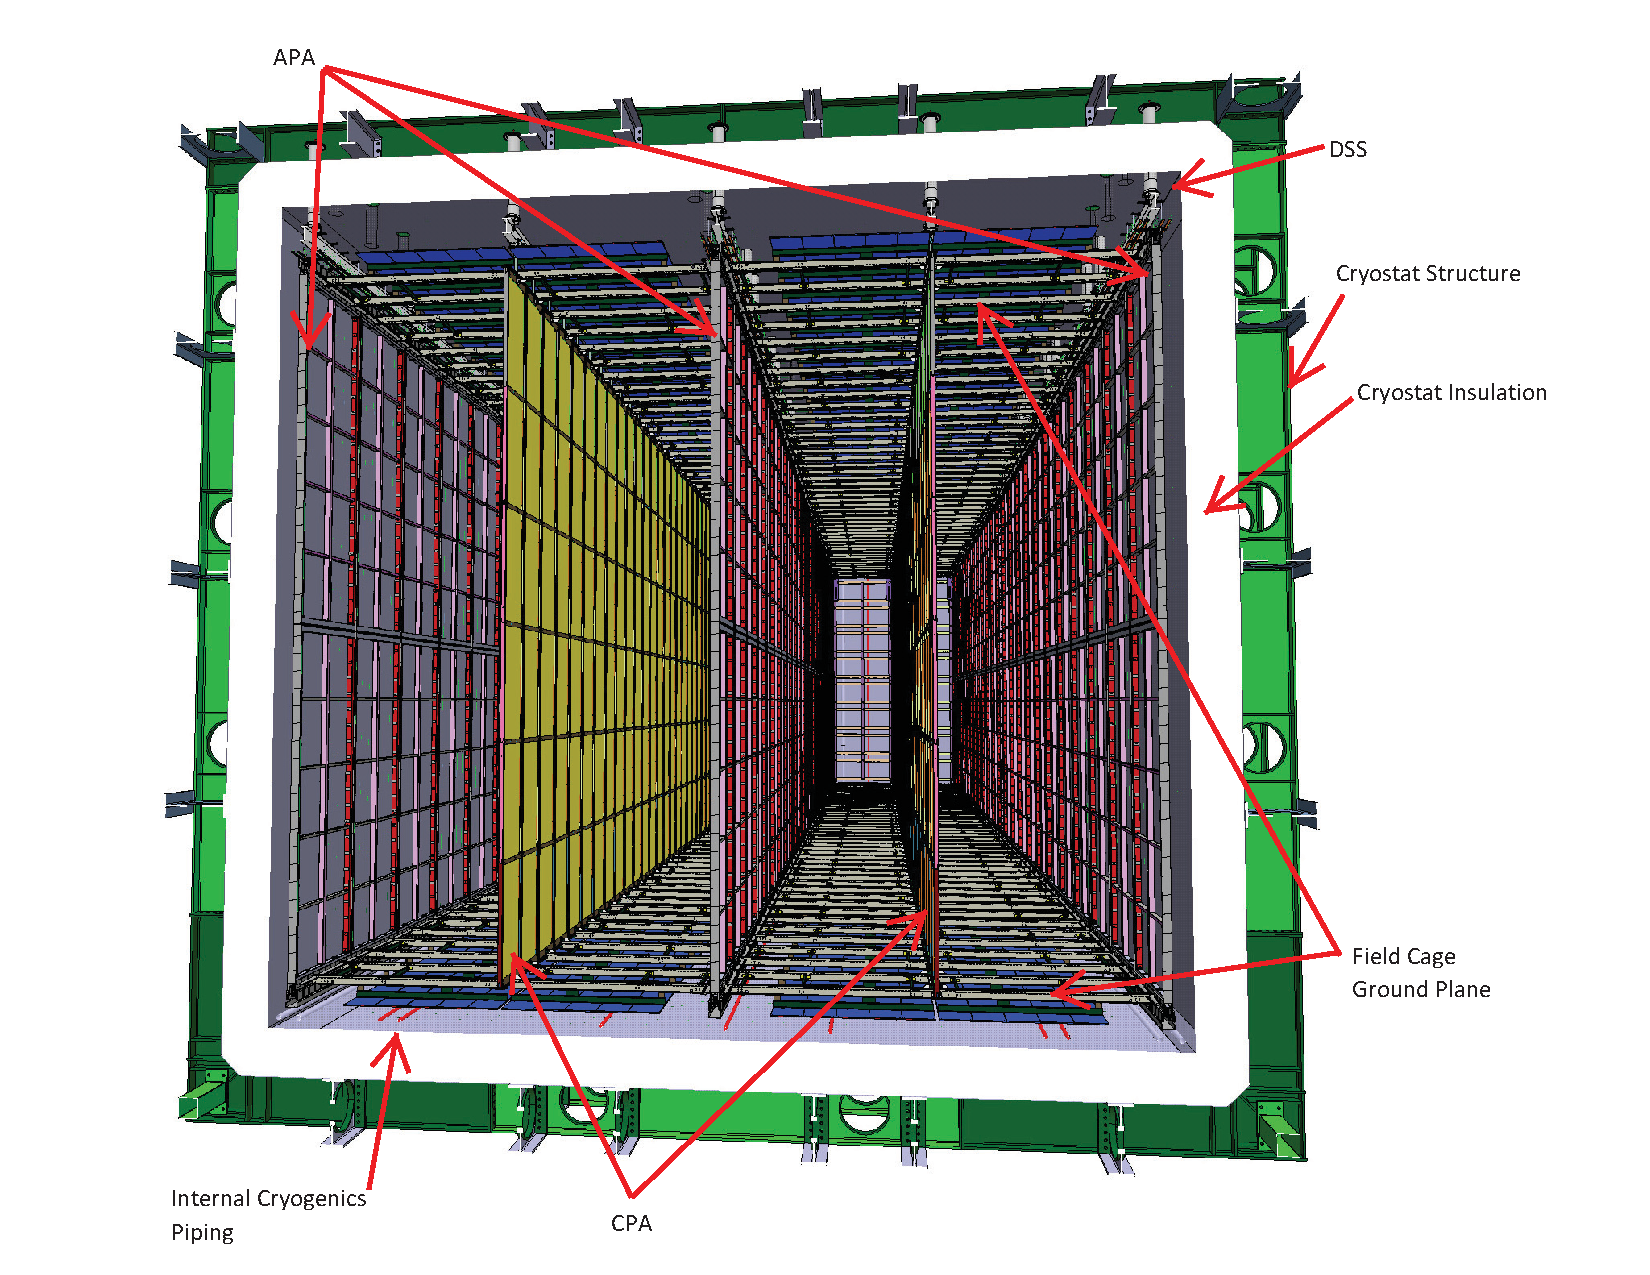
\includegraphics[width=0.99\textwidth]{DUN_SP_model.pdf}
\end{dunefigure} 

The module is contained in a cryostat with
internal dimensions of \SI{62}{\meter} long, \SI{15.1}{\meter} wide
and \SI{14}{\meter} high.  Four drift volumes are created between
alternating \dword{apa} and \dword{cpa} walls on sides, \dwords{fc} and
ground planes on top and bottom, and two end walls.  Each drift volume
is \SI{58.17}{\meter} long, \SI{3.52}{\meter} wide and
\SI{12.01}{\meter} high.  The entire assembly is supported from the
roof of the cryostat with \dword{dss}.

Each of the three \dword{apa} walls consists of an array of \num{25}
wide and \num{2} high individual \dwords{apa}, each with dimensions
of \SI{6.2}{\meter} high and \SI{2.32}{\meter} wide. There are
\num{150} \dwords{apa} in one module. Each \dword{apa} contains
\num{10} \dwords{pds}. Each of the two \dword{cpa} walls consists of an
array of \num{25} wide and \num{1} high individual \dwords{cpa}, each
with dimensions of \SI{12.1}{\meter} high and \SI{1.16}{\meter}
wide. There are \num{100} \dwords{cpa} in one module.  \dword{cpa}
walls are held at $-$\SI{180}{\kilo\volt}. With \dword{apa} walls held
close to ground, the result is a \SI{511}{\volt/\centi\meter} gradient
across the drift volume. The drift in the \dword{dsp} is in the horizontal 
direction. The \dword{lar} level is above the top set of ground planes and just
below the \dword{dss}.

Readout electronics are assembled on the \dwords{apa}. Cables from the
readout electronics and \dwords{pds} are routed to the cryostat roof
where they exit through a set of \num{75} feedthroughs. The cables are
connected to warm interface boards which are contained in \num{150}
crates for \dwords{apa} and \num{75} crates for \dwords{pds}. Data
fibers from the warm interface crates carry the data to DAQ racks
inside the \dword{cuc}.

There are four high-voltage feedthroughs on top of the cryostat, two on
each end. In addition, there are feedthroughs for calibration,
instrumentation and cryogenics distribution. Power supplies, and
controls are located on top of the cryostat on a dedicated
mezzanine. Cryogenic equipment are also installed on a separate
mezzanine on top of the cryostat.

\section{DUNE Dual Phase Far Detector Module}
\label{sec:fdsp-DP-module}

\fixme{Text below for dual phase is gleaned from DP IDR, it needs to be checked}

As with the \dword{dsp}, each \dword{ddp} LArTPC is a \SI{10}{\kilo\tonne} module,
contributing to the full \SI{40}{\kilo\tonne} Far Detector fiducial
mass.  One \SI{10}{\kilo\tonne} \dword{ddp} module is shown in
Figure~\ref{fig:DUNE_DP_model}.
\begin{dunefigure}[A \SI{10}{\kilo\tonne} \dword{ddp}
module.]{fig:DUNE_DP_model} {A \SI{10}{\kilo\tonne} DUNE Far Detector
    Dual Phase module.}
  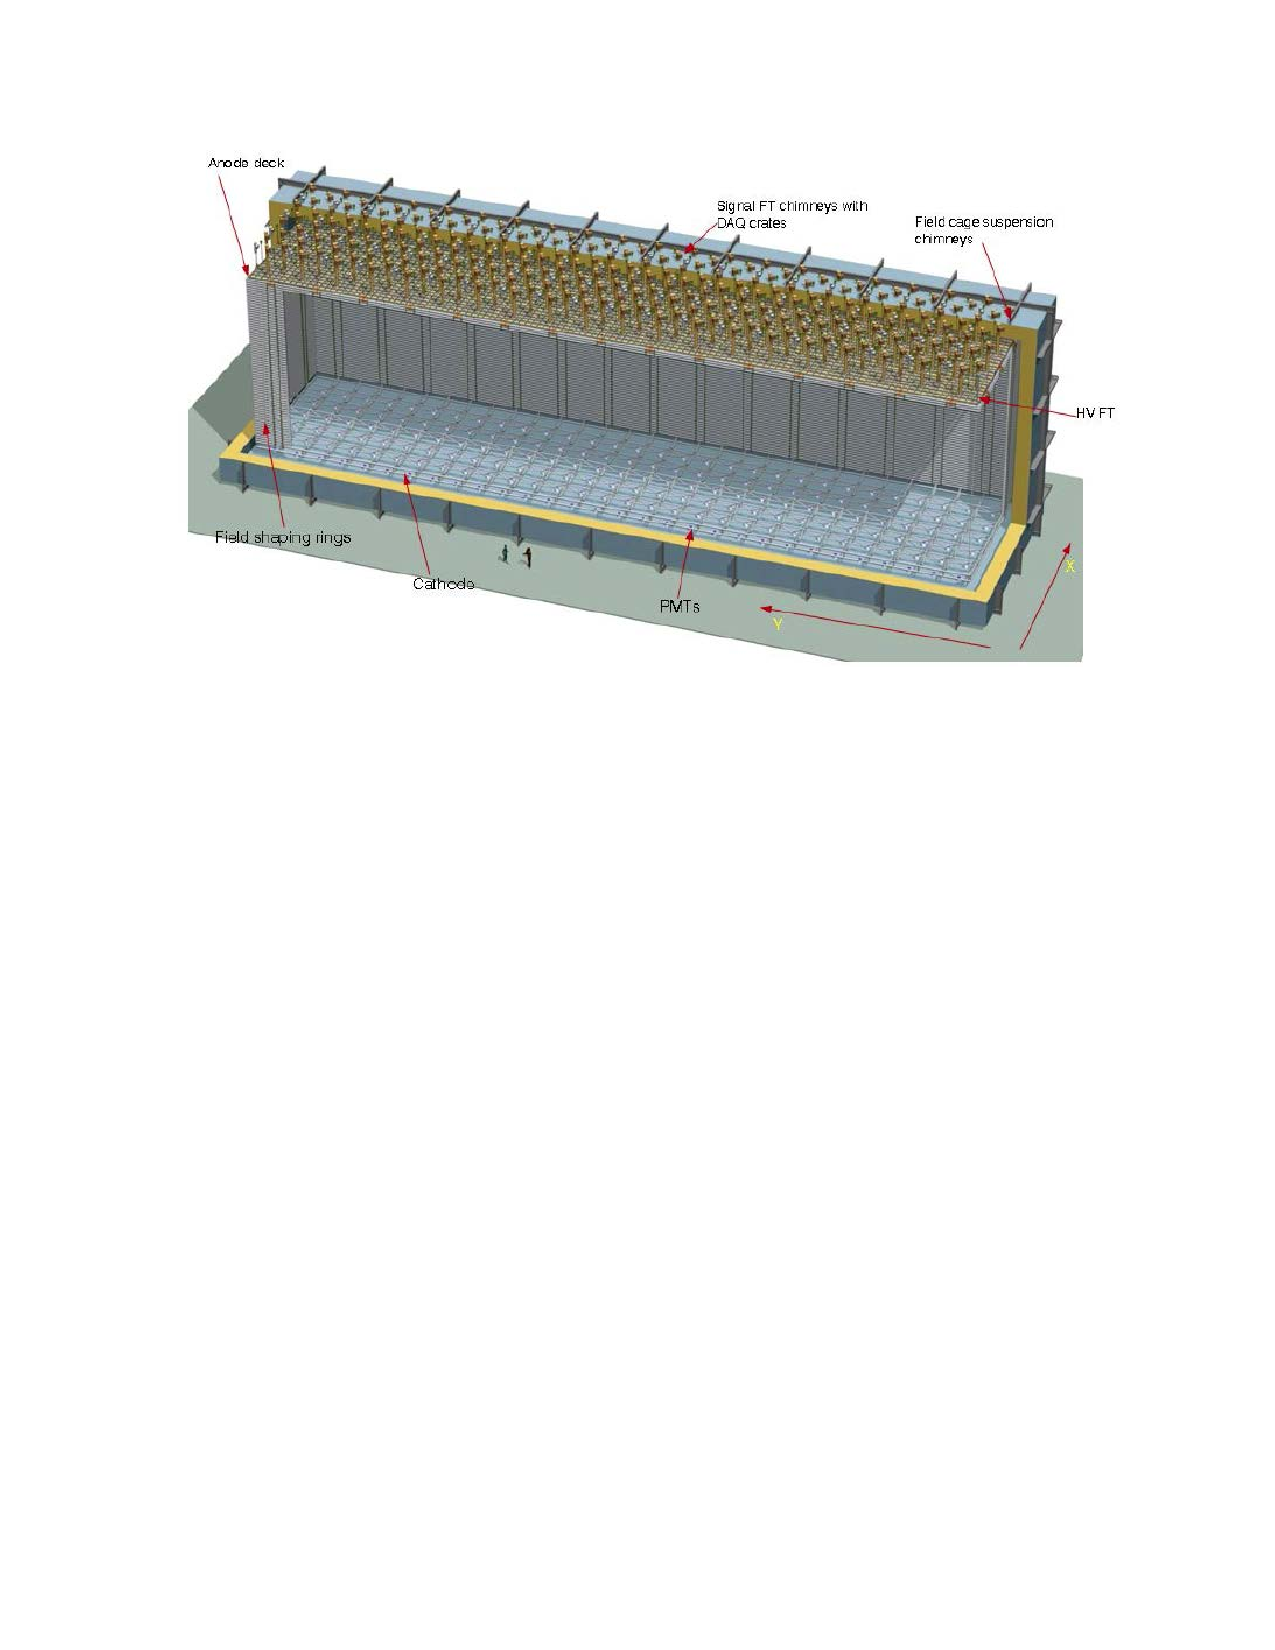
\includegraphics[width=0.8\textwidth]{DP-overview}
\end{dunefigure} 

Also as with \dword{dsp}, each \dword{ddp} module is contained in a
cryostat with internal dimensions of \SI{62}{\meter} long,
\SI{15.1}{\meter} wide and \SI{14}{\meter} high. But unlike the
\dword{dsp}, \dword{ddp} module consists of a single drift volume with
a vertical drift direction.

The drift volume is encompassed on the top by an array of \num{80}
\dwords{crp}, on the bottom by cathode planes and one the perimeter by
\dwords{fc}. It is \SI{12}{\meter} in height with a
\SI{500}{\volt/\centi\meter} gradient. The cathode is held at a
potential of $-$\SI{600}{\kilo\volt}. The \dword{ddp} \dword{pds}
consists of \num{000} \dwords{pmt} at the bottom of the drift volume
and is integrated with the cathode planes.  The \dword{lar} level in
\dword{ddp} module is within the \dword{crp}, just above the
collection grid and below the anode readout plane. A gradient of
\SI{2}{\kilo\volt/\centi\meter} in this region is used to extract the
drift electrons from the liquid. A \dword{lem} with a gradient of
\SI{33}{\kilo\volt/\centi\meter} causes charge multiplication and
amplification of the charge that  is then collected on the anode 
consisting of a @D set of two 3.125 mm-pitch gold-plated copper strips.

The \dword{ddp} \dword{dss} consists of a set of stainless steel
cables that are suspended from feedthroughs on top of the
cryostat. The cables are extended to the floor of the cryostat where
they are used to lift components to design height. In the case of
\dwords{crp}, there are three cables per panel with active height
control in order to postion the panel precisely with respect to the
\dword{lar} surface.

The cryogenic FE electronics is installed in the signal feedthrough
chimneys (SFT chimneys) on the roof of the cryostat to process the
LArTPC signals. Each SFT chimney is coupled to a microTCA crate to
digitize the signals. These crates are connected via optical fiber links to the DAQ
back-end. Arrangement of equipment on top of the cryostat is similar to \dword{dsp}.

\section{DUNE Far Detector Consortia}
\label{sec:fdconsortia}

A total of eleven Far Detector consortia have been formed to cover 
the sub-systems required for the two detector types currently under
consideration.  In particular, three consortia (SP-APA, SP-TPC
Electronics and SP-Photon Detection) pursue sub-systems specific to
the single-phase design and another three consortia (DP-CRP, DP-TPC
Electronics and DP-Photon Detection) pursue designs for dual-phase
specific sub-systems.  An additional five consortia (HV System, DAQ,
Cryogenic Instrumentation/Slow Controls, Calibration, and Computing)
have responsibility for sub-systems common to both detector
technologies.  Figure~\ref{fig:DUNE_consortia} shows the consortia 
associated with the far detector construction effort along with their 
current leadership teams.  

\begin{dunefigure}[\dword{dune} consortia]{fig:DUNE_consortia}
  {\dword{dune} consortia.}
  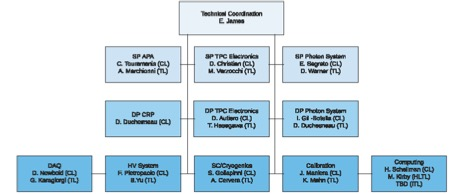
\includegraphics[width=0.99\textwidth]{DUNE_consortia}
\end{dunefigure}

\section{Work Breakdown Structure (WBS)}
\label{sec:fdsp-coord-wbs}

The complete scope of the DUNE construction project is captured in a 
\dword{wbs} to understand the distribution of deliverables between 
the consortia.  In combination with interface documentation, the 
WBS is used to validate that all necessary scope is covered.  The 
\dword{wbs} is also used as a framework for building \dword{dune} 
detector cost estimates.

The highest-level layers of the \dword{dune} \dword{wbs} are summarized 
in Table~\ref{fig:WBS_level2}.  At Level 1 the WBS is broken down into 
six elements corresponding to the five \dword{dune} detector modules (4 
far detector and 1 near detector) and \dword{tc}.  The scope documented
here is fully contained within the \dword{tc}, first far detector module 
(SP), and second far detector module (DP) Level 1 elements.   
\begin{dunefigure}[\dword{dune} \dword{wbs} at level 2]{fig:WBS_level2}
  {High level \dword{dune} \dword{wbs} to level 2.}
  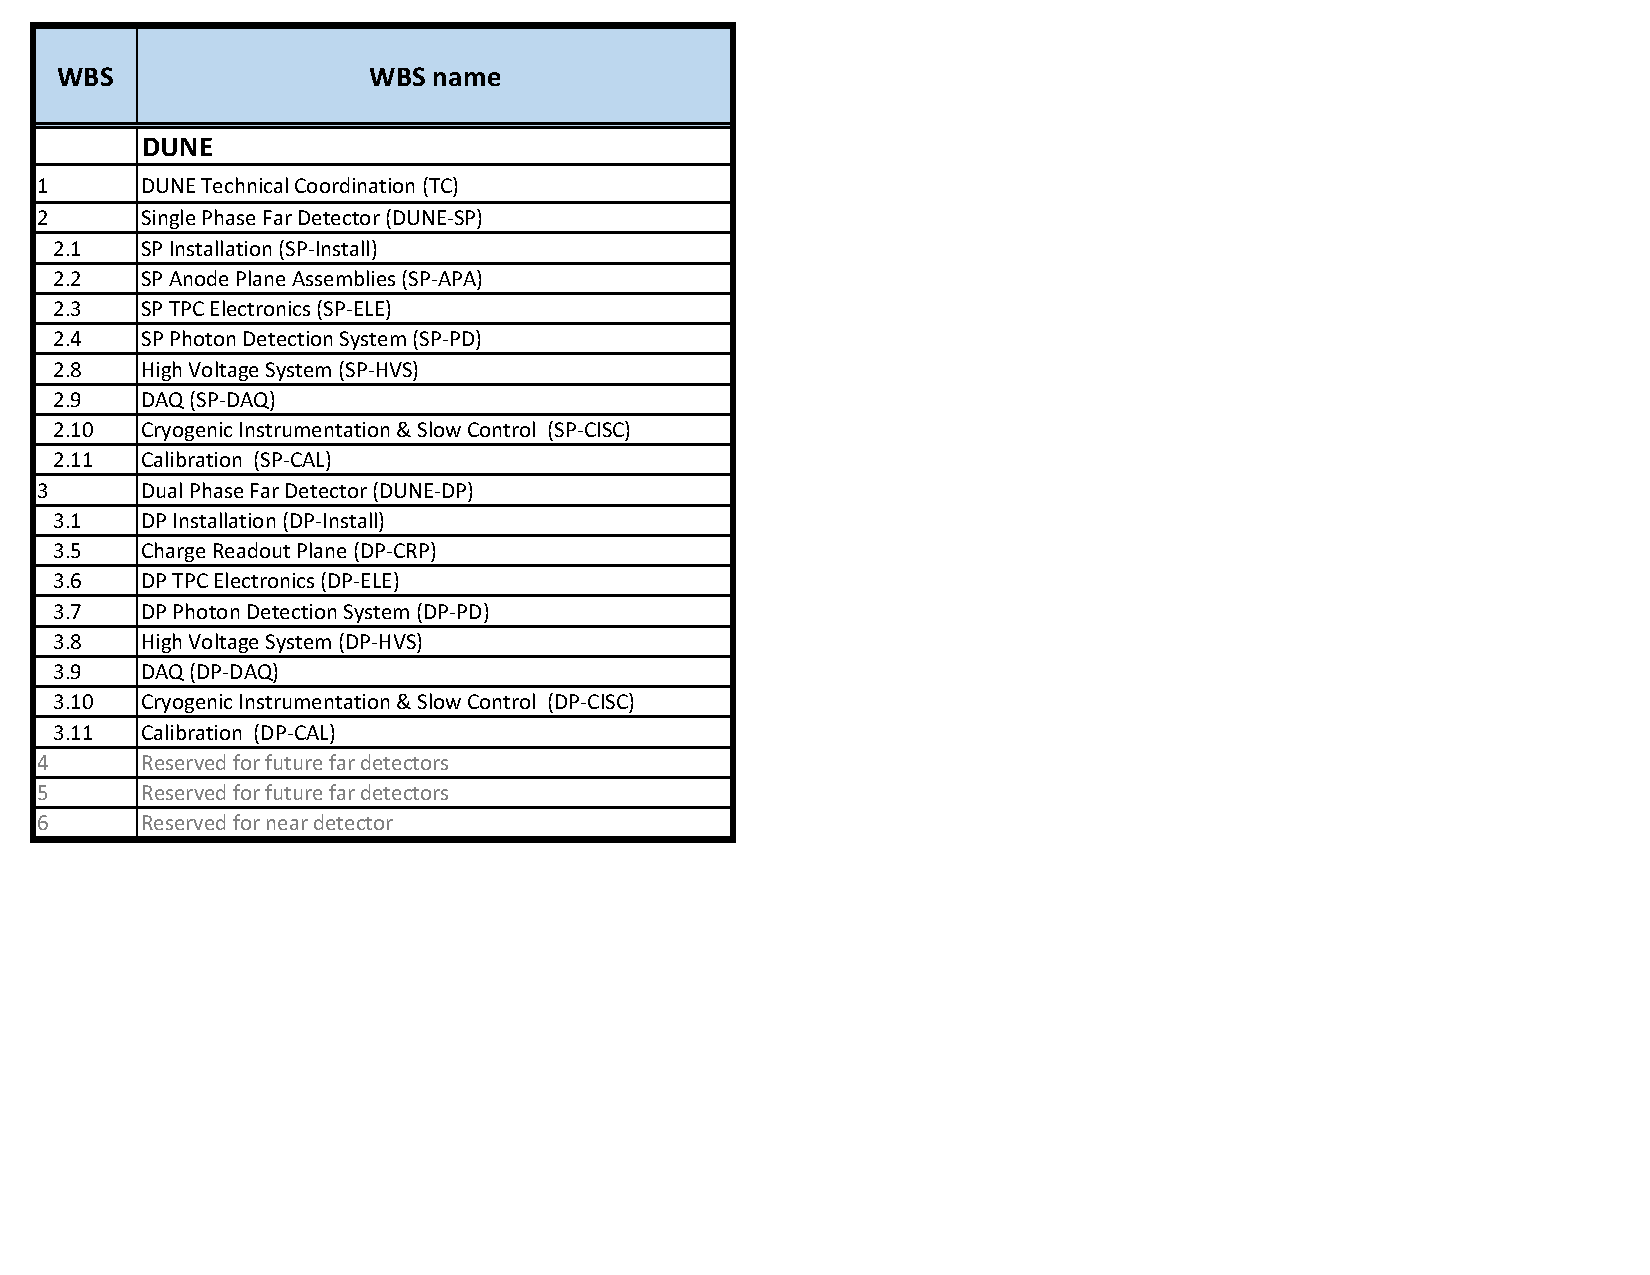
\includegraphics[width=0.75\textwidth]{WBS_level2_v2}
\end{dunefigure}

For the far detector module elements at Level 1, the \dword{wbs} breaks 
down at Level 2 into elements encompassing the deliverables provided by 
each consortium to that detector module along with an element containing 
common deliverables associated with the required detector installation 
and integration effort.  Since each consortium takes responsibility 
for a particular subsystem, this breakdown effectively corresponds to 
a division of deliverables across subsystems. 

The Level 3 breakdown of the Level 2 subsystem \dword{wbs} elements follow 
a common format that separates required activities into groupings defined 
roughly by their sequence in time.  A total of six elements are used as 
follows:     
\begin{enumerate}
  \item Management
  \item Physics and Simulation
  \item Design, Engineering and R\&D
  \item Production Setup
  \item Production
  \item Integration and Installation
\end{enumerate}
The groupings at Level 3 allow for the separation of costs associated with 
CORE and non-CORE activities and also of the costs associated with one-time 
and re-occuring activities in the case where two identical detector modules
are constructed.   

Lower-levels within these \dword{wbs} elements are determined by 
the responsible consortia and generally correspond at Level 4 to 
the different primary detector components from which each subsystem
is assembled.  This Level 4 structure is repeated under each of the 
Level 3 items to ensure that the full cost of each primary detector 
components can be rolled-up over the sequence of activities defining 
their design, production, and installation.       

\section{\dword{dune} Design Maturity}

The \dword{dune} project builds on significant development in previous
large \dword{lartpc} detectors (ICARUS and MicroBooNE) and on
substantial development from LBNE and LBNO. One of the most important
elements that has significantly advanced the project development is
the successfully construction and operation of the \dword{protodune}
detectors. These detectors use full-size \dword{dune} components and
processes. The construction of \dword{protodune} has established
teams, production lines, QA and QC processes, installation, operation
and performance of the final \dword{dune} detectors. Based on the
success of \dword{protodune}, \dword{dune} has reached advanced technical
maturity, approaching (80\%). The designs have significantly advanced
from \dword{protodune} to \dword{dune}. Most subsystems completed
\dword{pdr} or 60\% reviews on design modifications beyond
\dword{protodune} in advance of the \dword{tdr}. The overall level of
design maturity is now $\sim$90\%. The breakdown of the design maturity
level for \dword{dsp} by subsystem is provided in
Table~\ref{tab:designmaturity}. The table shows the final \dword{dune}
design maturity at the time of \dword{protodune} and now at the time
of the \dword{tdr}, along with the estimated design effort or weight
of each subsystem. The \dword{apa} conceptual design was developed in
2010 and prototyped at 40\% scale and again in the 35-ton detector. The version
deployed in \dword{pdsp} is close to that for \dword{dsp} (85\%). The
cold electronics low noise system design, including feedthroughs,
cables and grounding, was successfully prototyped at large scale in
MicroBooNE and \dword{pdsp} and is 90\% mature. The front end chip has
gone through eight iterations and was successfully demonstrated in
MicroBooNE and \dword{pdsp} (90\%). The frontend motherboard has gone
through a similar number of iterations and was successfully
demonstrated in \dword{pdsp} (80\%). The ADC chip has evolved from a
previous version used in CMOS 180~nm technology that was tested to $-50\circ$C. (50\%). Key
elements of the COLDATA chip have been prototyped (25\%). The HV
design has evolved from ICARUS, MicroBooNE and the 35-ton detector.  It
has been prototyped in subsequent runs of the 35-ton detector and
demonstrated in \dword{pdsp} (80\%). The photon system ARAPUCA design
has been prototyped at small scale and in \dword{pdsp} (20\%). The
mechanical design has been extensively developed using the 35-ton
detector and \dword{pdsp} (85\%). The DAQ artdaq backend has been
developed in several experiments, including the 35-ton detector and
\dword{pdsp}. The DAQ FELIX frontend has been developed by ATLAS and
prototyped in \dword{pdsp}.
\begin{dunetable}
  [\dword{dsp} design maturity]
  {|p{0.1\linewidth}|rp{0.1\linewidth}|rp{0.25\linewidth}|rp{0.2\linewidth}|}
  {tab:designmaturity}
  {\dword{dsp} design maturity}
  System & Weight & \dword{protodune} & \dword{dune}   \\ \toprowrule
  DSS & 10\% & 75\% &  85\% \\ \colhline
  APA & 30\% & 85\% &  95\% \\ \colhline
  CE  & 20\% & 80\% &  90\% \\ \colhline
  PDS & 10\% & 50\% &  65\% \\ \colhline
  HVS & 15\% & 80\% &  95\% \\ \colhline
  DAQ & 10\% & 60\% &  80\% \\ \colhline
  CISC & 5\% & 80\% &  90\% \\ \colhline \colhline
  Total& 100\% & 76\% & 90\% \\ \colhline
\end{dunetable}

The design maturity of the \dword{ddp} detector is also quite
advanced. It builds on working noble liquid \dwords{tpc} for dark
matter and neutrinoless double beta decay experiments. A significant
benchmark is the operation of the $3\times1\times1$ demonstrator at
CERN. A critical test will be the operation of \dword{pddp} at CERN. A
similar table of design maturity for \dword{ddp} will be included
here.

%%%%%%%%%%%%%%%%%%%%%%%%%%%%%%%%

